\chapter{Detector Characterization} \label{detector}

\section{Overview}
One of the core aspects of the LIFE instrument, along with the Fourier Transfer Spectrometer, is the Mercury Cadmium Telluride infrared detector. This detector images the atmosphere and blackbodies through the optical system and the FTS to create raw interferograms, which are saved to the computer. There are various parts of MCT detectors that must be carefully characterized so that the data is as optimized. The task of characterizing and optimizing the LIFE MCT detector forms the second part of this thesis. This chapter provides an overview of the MCT detector specific to the LIFE instrument in Section \ref{ABB_detector}, as well as the work originally done to verify the detectors nominal operation in Section \ref{detector_verif}. Afterwards, various measurements were taken in the lab to optimize a number of different components of the detector, which is described in Section \ref{detector_char}. This was all done prior to flight to optimize the data; Detailed post-flight analysis of the detector and the measured data is outside the scope of this thesis.

\section{LIFE Detector}\label{ABB_detector}
The LIFE MCT infrared detector was a custom purchase with the FTS from ABB, and is designed to function optimally with the LIFE system. It is manufactured by InFraRed Associates, and interfaces with the two custom amplification and digitization data acquisition (DAQ) boards also provided by ABB. The linear array of the MCT detector is 16 0.25\,mm\textsuperscript{2} square pixels, which respond to incident radiation from 2-14\textmu m, as is expected from an MCT-type detector. As described in Section \ref{IR_detector_types}, MCT detectors must be cooled to low temperatures to avoid saturation. The InFraRed Associates MCT Detector comes with an attached Stirling cooler manufactured by Ricor, which cools the pixels to 77K. The 16 pixels provide 16 interferograms, which are split into two groups of eight and sent to the two DAQ boards where the signals are amplified. The two boards are connected to a computer where the data is then stored. These specifications are all given directly to the LIFE research team by ABB. An image of the LIFE detector is in Figure \ref{fig:life_detector_from_ICD}.

\begin{figure}[h]
  \centering
  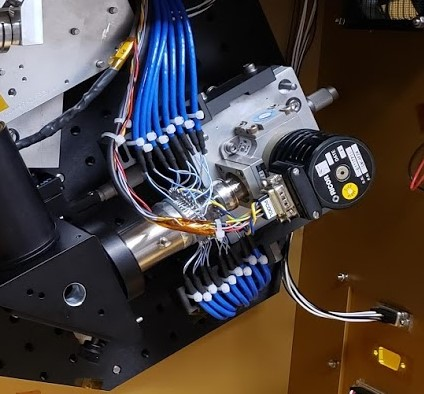
\includegraphics[width=0.6\linewidth]{chap5_images/detector_in_LIFE.jpg}
  \caption{Image of the MCT Detector in the LIFE instrument.}
  \label{fig:life_detector_from_ICD}
\end{figure}

\section{Detector Verification}\label{detector_verif}
Before the detector could begin to be characterized, work was done to ensure that the detector was operating as expected. This work, and other optimization work, needed to be done in-house as the detector was originally designed and programmed to run in a different mode than in the LIFE application, known as \textit{constant current} mode. In this mode, a constant current flows through the detector and a change in voltage is measured. In the ABB application in conjunction with the FTS, \textit{constant voltage} mode is used. Here, the a constant voltage known as the \textit{bias voltage} flows through the detector, and a current change can be measured. Also, verification tests allowed familiarization with the detector and its various settings before attempting optimization. These tests were completed with the lab version of the instrument; i.e. they were completed with the MCT and FTS mounted on an optical bench rather than in the flight configuration. This was not ideal, as the system was not as well aligned as in the flight configuration, but it suffices for the optimization necessary. Tests were planned to be completed in flight configuration as well, but due to troubleshooting leading to the launch and damage sustained during the descent, these were not able to be completed.

To perform all verification and optimization work, there are two particular settings that can be changed via software for the LIFE MCT detector: The bias voltage, as described previously, and the offset current. The offset current raises and lowers the baseline of the measured current, and should be altered so that it does not dip below zero or saturate. These settings are related to the raw ADC output value of the detector through Equation \ref{ADC_output_ABB} and \ref{ADC_I_detector}, which are specific to the LIFE system as provided by ABB.

\begin{equation} \label{ADC_output_ABB}
    ADC_{raw\:value} = \frac{(I_{detector} + I_{offset})(-G)(2^{24}-1)}{ADC\:Voltage\:Reference\:Range}
\end{equation}

\begin{equation} \label{ADC_I_detector}
    I_{detector} = \frac{V_{bias}}{R_{detector}}
\end{equation}

For the case of the LIFE MCT detector, the ADC Voltage Reference Range is 4.096\,V, and R\textsubscript{detector} is a function of the incident infrared optical signal flux. This function is typically linear, and for the LIFE detector over the expected operating range can be assumed to be a constant 50 {\textOmega} as recommended by ABB. However, as this is only an approximation, it is a source of some non-linearity that must be considered. G is the combined gain of all amplifiers, given as 195.65 V/A by ABB. As much of Equation \ref{ADC_output_ABB} is made up of constants, it is easier to look at the proportional relationship between the ADC values and the bias voltage and offset current, shown in Equation \ref{ADC_output_proportional}.

\begin{equation} \label{ADC_output_proportional}
    ADC_{raw\:value} \propto -\left(\frac{V_{bias}}{R_{detector}} + I_{offset}\right)
\end{equation}

With this simplified equation it is easier to see the dependencies. This forms a simple slope formula, with the bias voltage as the slope and the offset current as the y-intercept. Thus the operation of the detector can be verified by taking various measurements with changing bias and offset settings. Numerous measurements were taken with the detector of blackbodies, and python software was developed to read these measurements to determine the output of the MCT system. It is noted that the output data presented in these tests is known as the \textit{DC Component}, or the mean of the data, over an entire scan of the blackbody. This DC Component value is the same as the theoretical ADC raw value from Equation \ref{ADC_output_proportional}.

Before changing the bias and offset settings, a simple test was done of taking images of a blackbody with a temperature changing from 25°C to 60°C in 5°C increments. This was done to see the ADC output change based on blackbody temperature, giving an idea of the ADC range with different temperatures and the general output of the system. The result is shown in Figure \ref{fig:ADC_dep_on_bb_temp}.

\begin{figure}[h]
  \centering
  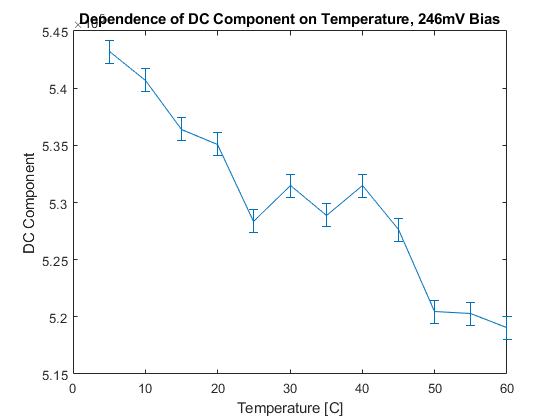
\includegraphics[width=0.8\linewidth]{chap5_images/DC_dep_on_temp.png}
  \caption{The result of changing the blackbody temperature on the raw detector signal.}
  \label{fig:ADC_dep_on_bb_temp}
\end{figure}

This plot shows that there is a negative temperature dependence in the output data, which is a feature of the detector to avoid detector saturation at high temperatures. This allows the interferogram and detector to avoid saturation while more of the detector temperature range can be used. This result was helpful, as it also led to explanations of values for responsivity, which is described in Section \ref{responsivity_sec}.

Beyond the overall decrease in the plot, ideally this should be much more linear. It was theorized that during the tests, the ambient temperature of the room had an effect on the output data. An air conditioning unit in the lab room and near the instrument cycled often, which would cause differing ambient temperatures throughout a test. This ambient temperature could affect the blackbody surfaces that were being imaged, as well as the surface of parts of the instrument that were possibly being imaged due to misalignment. A test done by taking images of the blackbodies at a constant temperature over a period of a few hours confirmed that the ambient temperature changes were having an affect on the output data, the results of which is shown in Figure \ref{fig:ADC_dep_on_room_temp}.

\begin{figure}[h]
  \centering
  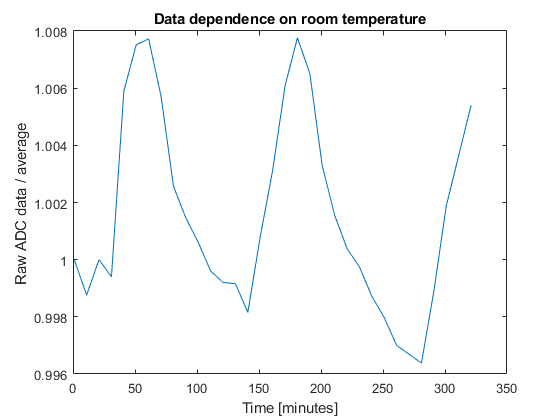
\includegraphics[width=0.8\linewidth]{chap5_images/DC_dep_on_room_temp.png}
  \caption{The result of the ambient room temperature changing throughout a longer term test, causing temperature changes in the blackbodies.}
  \label{fig:ADC_dep_on_room_temp}
\end{figure}

Although this is an issue that affects the lab data, it is unlikely to occur in the flight configuration of the instrument, as it was designed to be better thermally controlled as well as properly aligned. Ideally this would have been tested further after flight but as mentioned previously there was no opportunity. 

Once these initial measurements were taken, further verification using the bias and offset settings could continue. Two main tests were done, one with constant bias voltages and incrementing offset current, and vice versa. For both tests, specific values were chosen for the constant bias voltage or offset current, respectively. These values were taken from a calibration spreadsheet provided by InfraRed Associates. As stated previously, the calibration would not work for the LIFE application due to it operating in a different mode, but there were specific values chosen for the bias voltage and offset current for all calibration tests; these are shown in Table \ref{vbias_ioffset_table}. As there were a very wide range of possible settings, it was assumed that these values would be reasonable to begin with as they had been chosen by the manufacturer. 

\begin{table}[h]
\begin{center}
\begin{tabular}{ |c|c| } 
 \hline
 \rowcolor{lightgray}
 Bias voltage $V_{bias}$ [mV] &  Offset Current $I_{offset}$ [mA]\\ 
 \hline
  246 & 4 \\ 
  \hline
 431 & 6  \\
 \hline
 625 & 8 \\
 \hline
 \end{tabular}
\end{center}
\caption{Bias voltage and offset currents as used in the factory calibration, used here as a baseline.}
\label{vbias_ioffset_table}
\end{table}

Measurements were done by taking images of a hot blackbody at 50°C and a cold blackbody at 10°C for both tests. For the first test, the offset was chosen as three constant values based on the factory calibration, and the bias voltage was incremented over a range chosen as 0.1\,V to 1\,V in 0.1\,V steps. The resulting data is shown in Figure \ref{fig:dc_dep_on_bias}. It is noted that the detector was not constrained to the voltage range above, this was based on calibration values. It was noted by ABB that the range was much larger and there was no danger of destroying the detector with different values, but it was found that beyond this range there was no useful data and all tests were completed with these values.

\begin{figure}[h]
  \centering
  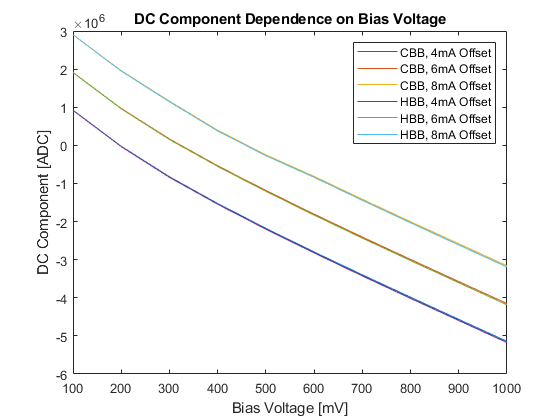
\includegraphics[width=0.9\linewidth]{chap6_images/verification/dc_component_dependence_on_bias_voltage.png}
  \caption{Detector raw data output dependence on bias voltage.}
  \label{fig:dc_dep_on_bias}
\end{figure}

The resulting dependence is expected. For each bias there is a small change in slope in the linearity of the data, as is expected from Equation \ref{ADC_output_proportional}. It is also downward sloping due to the negative proportionality, which results from the negative gain in the equation. The lines are all separated by the offset current chosen, also as expected. For each offset current, the cold blackbody measurement and blackbody measurement appear to overlap. However, if the plot is magnified, the cold blackbody data is slightly higher than the hot blackbody data, which matches what would be expected from \ref{fig:ADC_dep_on_bb_temp}; the cold blackbody produces a higher ADC signal due to the signal inversion as described previously. The fact that the lines overlap shows the major effect that altering these settings have on the data; the change in ADC measurements from looking at two different blackbody temperatures is an order of magnitude smaller than the change in ADC measurements from altering settings. Overall, this plot confirms Equation \ref{ADC_output_proportional}. Figure \ref{fig:dc_dep_on_offset} shows the second test, where the offset current is incremented over a range of 1\,mA to 10\,mA, with three bias voltages set according to factory calibration values. As with the bias voltage, the range of the offset current is much larger, but the aforementioned range was chosen to match the range of calibrated values.

\begin{figure}[h]
  \centering
  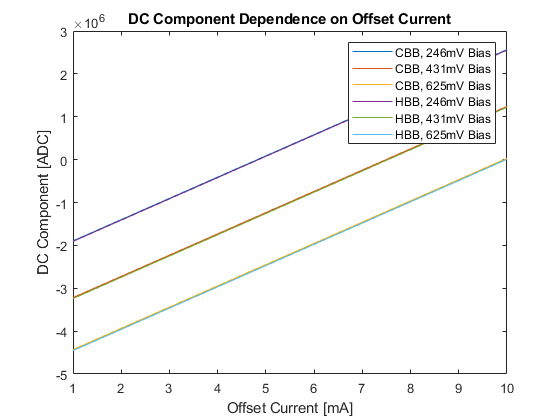
\includegraphics[width=0.9\linewidth]{chap6_images/verification/dc_component_dependence_on_offset_current.png}
  \caption{Detector raw data output dependence on offset current.}
  \label{fig:dc_dep_on_offset}
\end{figure}

The results shown in Figure \ref{fig:dc_dep_on_offset} are also as expected. The data is very linear with increasing offset current, and are split by different bias voltages. The slope is also slightly different for each plot, showing that the bias voltage does not have as large an impact on where the data is in the DC Component range. This would make sense as the function of the offset current is to move the baseline of the data, and the bias voltage is used to tune the responsivity; the results of changing this become more clear when tuning for responsivity. This is the topic of Section \ref{responsivity_sec}.

Overall, the results of changing the bias and offset settings on the output data match the equation provided by ABB that describes the system. Thus, the detector is verified to be working properly and as expected, and there is a greater understanding of the effect of altering the settings. Higher level optimization of the detector can now take place.

\section{Characterization}\label{detector_char}
To be able to produce the most accurate data possible, the MCT detector needs to be optimized to reduce common problems with MCT detectors such as non-linearity, and to detect incoming signal as well as possible. The latter corresponds with responsivity, which is discussed first and is the main characteristic to be optimized. A discussion of the calculation method, based on the GLORIA method, is described. A discussion of non-linearity follows, and the methods used to determine this, but the measurements and post-flight calibrations of non-linearity are out of the scope of thesis.

\subsection{Responsivity}\label{responsivity_sec}
Responsivity is the measure of how sensitive, or responsive, the detector is to incoming signal. It is typically in units of $ADC/Wcm^{-1}$, with the length component coming from the spectral dependence, but the spectral dependence can be integrated out if the wavelength limits are known, which they are for a known detector and measured temperatures. Thus the units of responsivity for the case of LIFE are $ADC/W$, which gives a direct conversion from the input photon counts to power, i.e. the change in power from the input photons, which can easily be converted to the change in current that is measured. Theoretically, a higher responsivity would mean better performance, as the counts measured by the detector cause a larger change in the output current and giving a more accurate reading~\citep{GLORIA_PhD}. However, if this change is too large, it can lead to non-linearity.

The responsivity is determined from an equation developed for the GLORIA instrument, which gives another equation for the raw output signal, similar to Equation \ref{ADC_output_ABB} from ABB. The GLORIA equation is based on measurement results from hot and cold blackbody systems. A blackbody system consisting of three blackbodies, one at a hot temperature, one at a warm temperature, and one at a cold temperature, was procured for this purpose. It is on-board the LIFE instrument so these can be used to calibrate the FTS during flight, as described in Chapter \ref{thermal}. The DC signal measured by the detector is given in Equation \ref{GLORIA_DC_signal_eq}.

\begin{equation} \label{GLORIA_DC_signal_eq}
    DC = A_{pix}\Omega_{pix}\int\limits_{\sigma_{min}}^{\sigma_{max}}\tau_{EW}(\sigma)\mathcal{R}_D(\sigma)L(\sigma, T)d\sigma
\end{equation}

Here $\sigma_{min}$ and $\sigma_{max}$ are the lower and upper cutoff wavenumbers, $A_{pix}\Omega_{pix}$ is the throughput of the system, $\tau_{EW}$ is the transmittance of the detector window, $\mathcal{R}_D$ is the detector responsivity, $L$ is the spectral radiance, and $T$ is the temperature of the blackbody. Whereas Equations \ref{ADC_output_ABB} and \ref{ADC_I_detector} are given by ABB and based on the detector and its design only, giving raw output data, Equation \ref{GLORIA_DC_signal_eq} shows a theoretical output of the entire system, including both detectors and optics. In addition, the method for calculating responsivity using Equation \ref{ADC_output_ABB} was not given by ABB and would require more work and characterization to determine a method. As the GLORIA system is similar to LIFE, Equation \ref{GLORIA_DC_signal_eq} applies to LIFE as well and is an accurate way of determining responsivity.

Using this equation at hot and cold temperatures, assuming the transmittance of the detector window to be unity, and rearranging, the detector response can be calculated from Equation \ref{rearranged_GLORIA_Resp}.

\begin{equation} \label{rearranged_GLORIA_Resp}
    \mathcal{R}_D = \frac{DC_{hbb} - DC_{cbb}}{A_{pix}\Omega_{pix}(L(T_{hbb})-L(T_{cbb}))}
\end{equation}

Here $DC_{hbb}$ is the DC component of the interferogram signal from the hot blackbody, $DC_{cbb}$ is the DC component of the interferogram signal from the cold blackbody, $L(T_{hbb})$ is the Planck function integrated over the range of wavenumbers for the hot blackbody, and $L(T_{cbb})$ is the Planck function integrated over the range of wavenumbers for the cold blackbody~\citep{GLORIA_PhD}. 

Now that there is an equation for the responsivity of the detector that can be related to the signal output, it can be tested with different inputs and settings on the detector. For all tests, the cold blackbody temperature was set to 10°C and the hot blackbody temperature was set to 50°C. Thus the responsivity between tests was entirely dependent on the DC signal from the hot and cold blackbodies, which the behaviour of is known from tests done in Section \ref{detector_verif}. The same bias voltage and offset ranges were used as the verification tests, and the first test of the responsivity dependence on offset current is examined. The results of these tests as calculated by Equation \ref{rearranged_GLORIA_Resp} are shown in Figure \ref{fig:resp_dep_on_offset}.

\begin{figure}[h]
  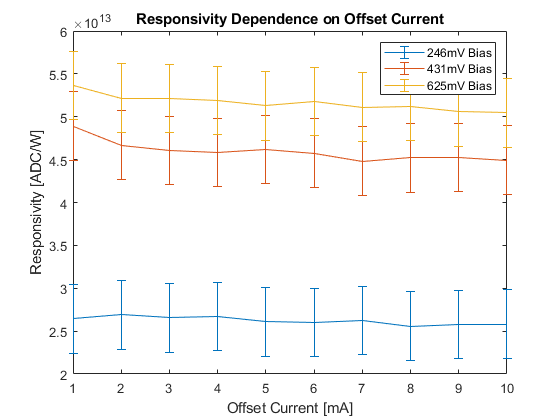
\includegraphics[width=\linewidth]{chap6_images/verification/resp_dependence_on_offset.png}
  \caption{Detector responsivity change with different offset settings.}
  \label{fig:resp_dep_on_offset}
\end{figure}

Figure \ref{fig:resp_dep_on_offset} shows that the offset current has little effect on responsivity, with data for each bias voltage being effectively linear. The spacing between each set of data shows the large effect that changing bias has on the data. Now that it is known that the offset current only has the effect of changing the baseline of the data but not the responsivity, the result of changing the bias voltage will be examined. It is done over a range of 100\,mV to 1\,V and is shown in Figure \ref{fig:resp_dep_on_bias}.

\begin{figure}[h]
  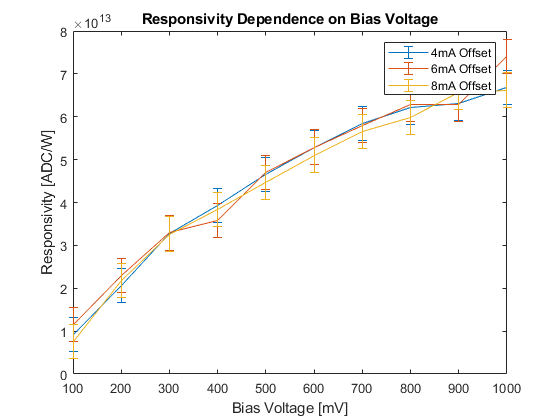
\includegraphics[width=\linewidth]{chap6_images/verification/resp_dependence_on_bias.png}
  \caption{Detector responsivity change with different bias voltage settings.}
  \label{fig:resp_dep_on_bias}
\end{figure}

This plot shows what is theorized; as the bias voltage increases, the responsivity of the detector increases. Also, the lines all effectively overlap, confirming Figure \ref{fig:resp_dep_on_offset}, showing that the offset current will not have an effect on the final value for responsivity. As mentioned before, theoretically, the responsivity should be as high as possible for the best detector performance, meaning that the bias voltage should be chosen to be at least 1\,V. However, there is a saturation limit on the bias voltage, where the detector will not operate correctly. This leaders to non-linearity, which can be seen in this plot. The increase in responsivity with bias voltage begins linear but slowly begins to decline as it reaches saturation levels. Further tests in the thermal vacuum environment would show that if the bias voltage became too high, leading to a high responsivity, the detector would not be able to dump enough heat to keep the temperature to 77K. Even after lowering the bias voltage, the detector took almost 2 hours to cool back down to its previous temperature. Thus the final value for bias voltage must be chosen so that is not so close to the non-linear range as to saturate and effect the data.

After examining the data, it was determined that with a bias voltage any higher than 500\,mV, there is a risk of non-linearity due to bias voltage having a large effect. Thus a bias voltage of 431\,mV was chosen, one of the values originally given by the manufacturer. The gains in responsivity past this point were not worth the chance of saturation, and as it was in the middle of the manufacturer's calibration range it seemed to be a good choice. Similarly, the offset current was chosen to be 6\,mA, in the middle of the manufacturer's calibration range. As the offset current had little effect on responsivity, this was set more to choose a middle baseline for the current range. These two settings were used for all pre-flight calibration measurements as well as the flight itself.

Further examination into the responsivity was planned after the instrument was in full flight configuration as well as after the flight, to research more closely the responsivity of the detector for each pixel and to examine the effect of non-linearity further. It would also help to inform the design for future versions of the instrument. However, due to the damage the instrument and particularly the detector sustained upon landing, this will not be possible. It is an important aspect of the instrument to examine if a second version of the instrument is planned or if the detector is fixed.

\subsection{Non-linearity}\label{non-linearity_sec}
The non-linearity of the LIFE system must be determined to allow for its correction and removal from the data. The non-linearity will have an effect on Equation \ref{ADC_output_proportional}, as based on the structure of this equation the results should be linear. There are a number of ways to determine the non-linearity of the system, which must be utilized to allow for its removal. There are two main sources of non-linearity in the LIFE system: Electrical, based on the electronics of the MCT and its settings, and optical, which is more dependent on the characteristics of the MCT itself as well as the design of the optical system.

The non-linearity due to the electrical system is characterized and removed through the altering of the bias voltage and offset current settings, which is largely described in the previous section. The non-linearity of this nature comes from the non-linear bias voltage of the detector, as well as the non-linear amplifier response in the amplifying circuitry of the data acquisition system. Nothing can be done about the amplifier non-linearity, but the settings can be chosen to remove the effect of non-linear bias voltage as much as possible. As described in Section \ref{responsivity_sec}, the responsivity curve is highly non-linear, due to the increasing bias voltage. This should be set as low as possible while still maintaining a high responsivity to mitigate this effect. The electrical non-linearity was minimized through these verification and responsivity characterization tests.

Non-linearity due to other parts of the system is more complex, making it more difficult to measure and more difficult to remove. A method of measuring the effect of non-linearity due to the optics is to measure the out-of-band spectral response. Here, signal can be seen in the resulting spectra outside of the cutoff wavelengths, where the measurement should be zero. There are different methods for characterizing this response, one of which is to examine a very cold blackbody. Theoretically, with a cold enough blackbody, there should be effectively zero signal measured by the detector. This was accomplished by examining a blackbody surface with a temperature dropped via liquid nitrogen to -100°C. This test needed to be done in a thermal vacuum chamber, so that frost would not build up on the blackbody surface; this would have changed the emissivity of the surface. Even though it was done in a vacuum environment frost was still an issue, but measurements were taken. The signal that was measured from the cold blackbody is the non-linearity, or the out-of-band response~\citep{non-linearity_correction}. This also helped to determine if any part of the system was being imaged due to misalignment which would cause a higher temperature than expected. This self-emission and out-of-band signal could be then be removed from the data. No further work could be done to optimize the instrument prior to flight, and the non-linearity signal would have to be removed from the flight data. Post-flight, the data is being analyzed by Ethan Runge for his PhD thesis, which includes further research into removal of the non-linearity from the flight data.

\section{Summary}
This chapter discusses the second part of this thesis, the characterization of the MCT detector. The detector used in the LIFE instrument is first described in detail, with the information given from the manufacturer. The initial work done for the verification is then described, which involved multiple tests to ensure that the detector was working properly prior to the characterization tests. The two main settings for the detector, offset current and bias voltage, were changed both for verification and to examine the detector responsivity and non-linearity, before attempting to improve these.

The characterization of the detector involved working with these settings to optimize the responsivity of the detector to provide the best measurements possible, while avoiding any non-linearity in the resulting data. A number of tests were done with different settings to find the best responsivity, and once a value was chosen it was used for all future tests. Non-linearity was examined in more detail, however most of this work is outside the scope of this thesis, along with the post-flight analysis.